\section{What is Upkeeper.}\label{index_whatis}
Upkeeper is a process control, monitor, with auditing system.

Upkeeper consists of 4 logical components
\begin{DoxyItemize}
\item Buddy -\/ The individual process monitor.
\item Controller -\/ The audit and control service.
\item Libupkeeper -\/ The client library.
\item Clients -\/ tools and utilities to interact with upkeeper.
\end{DoxyItemize}

upkeeper's is almost between DJB's daemontools, and freedesktop's systemd, in terms of functionality and capabilities. However, it adds the additional capability of recording state changes of monitored processes to a data store, which can then be interogated, preferably via the API, for the purpose troubleshooting, event correlation, metrics collection, trending, and analysis.\section{How the system works:}\label{index_howitworks}
A high-\/level view of the interaction between components is as follows:

\begin{center}

\begin{DoxyImageNoCaption}
  \mbox{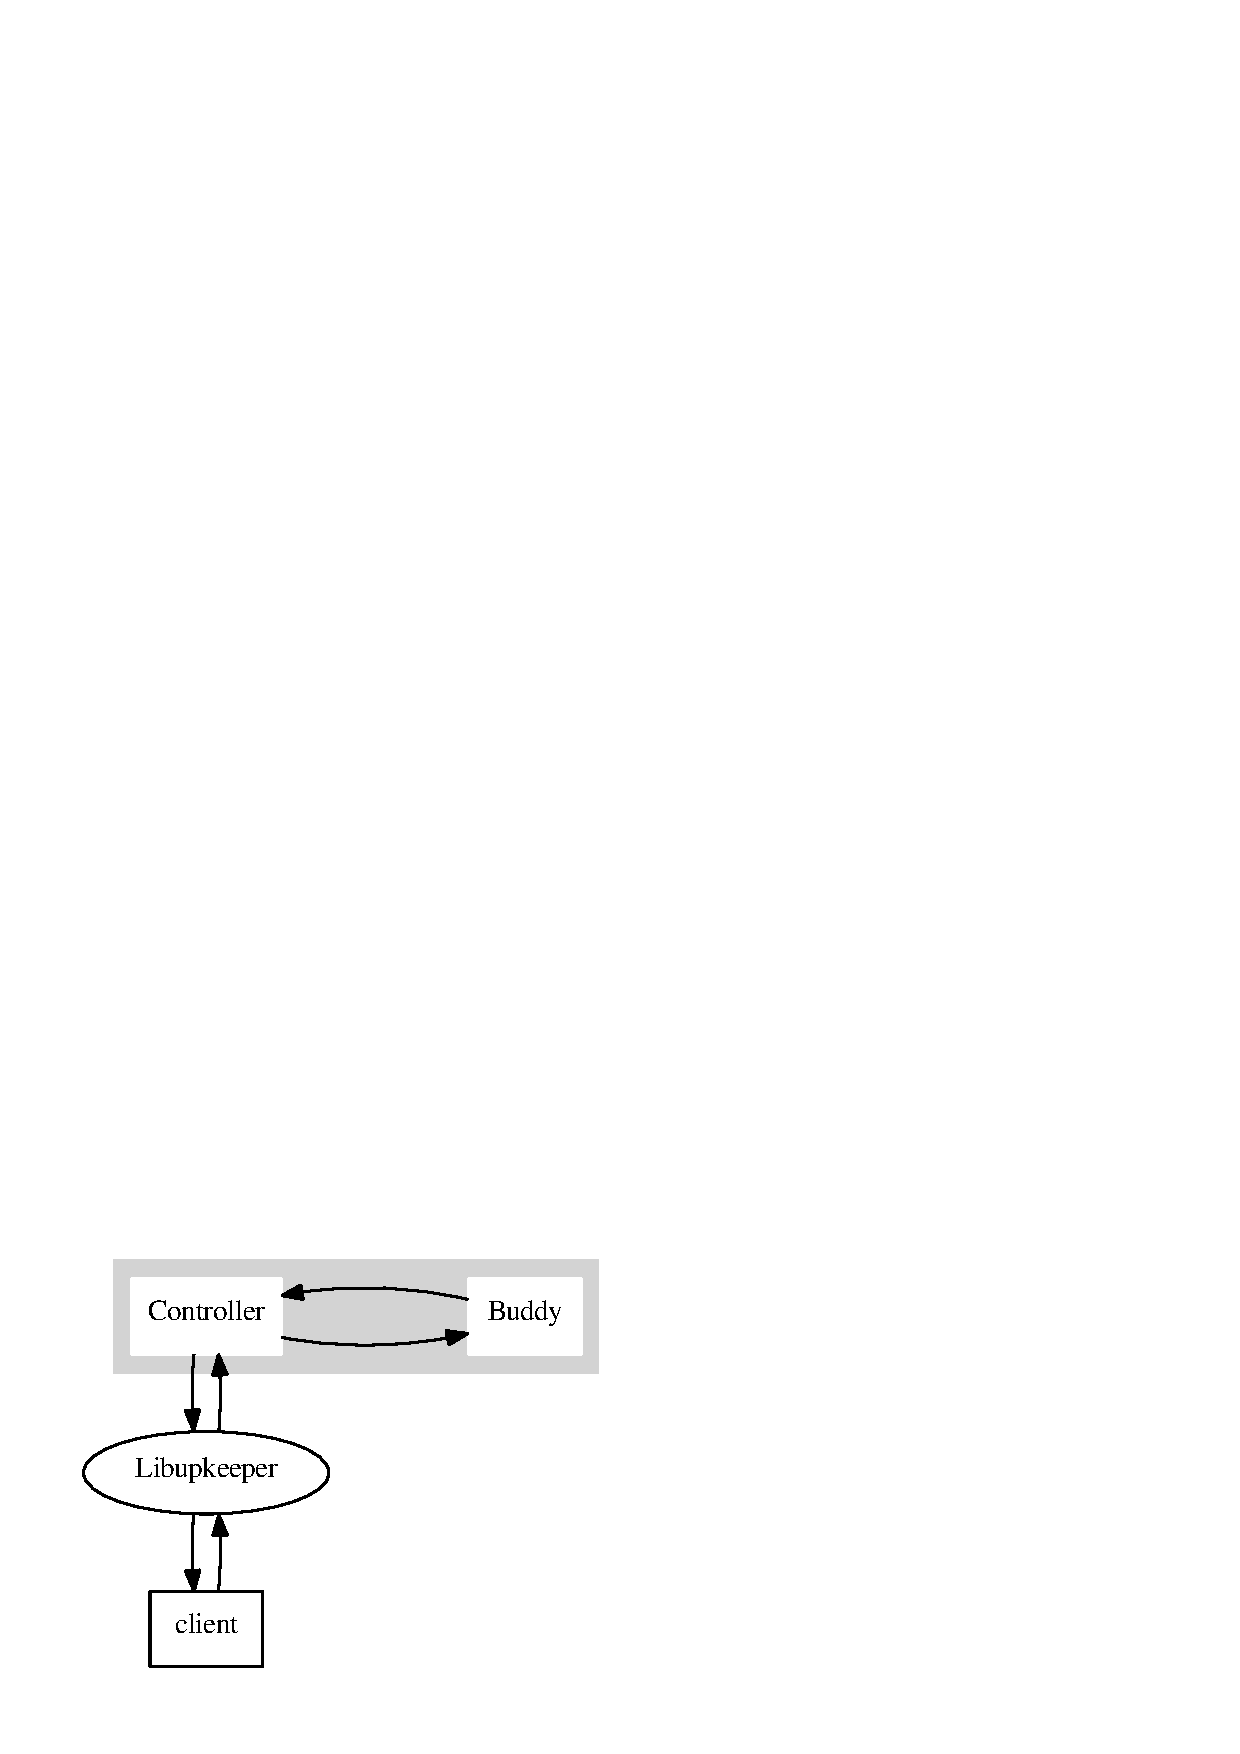
\includegraphics[width=\textwidth]{dot_inline_dotgraph_1}}
\end{DoxyImageNoCaption}
\end{center}


Controller is responsible for maintaining the configuration of buddy process, establishing the environment in which buddy runs, and invoking buddies. Once a buddy has been invoked, it runs autonymously until terminated. Excessive care has been taken to ensure that a buddy will not terminate under normal, and even some rather extraordinary, circumstances.

Buddy is a simplistic-\/by-\/design component that primarily just sits in a loop and waits for the process its monitoring to change terminate, or otherwise catch a signal. To communicate status changes with controller, buddy listens to a socket, which controller polls at a configurable interval. If controller dies for some reason, buddy has a user-\/configurably sized ringbuffer which will backlog status events, and report them once a controller becomes available. If a ringbuffer becomes $>$= 75\% full, or if a buddy is attempting to terminate while having events in its ringbuffer, the buddy will attempt to contact a controller on the controller's domain socket, as a last-\/resort.

The environment buddy runs in is a directory structure with files and symlinks that buddy uses to invoke actions, and log output. \begin{center}

\begin{DoxyImageNoCaption}
  \mbox{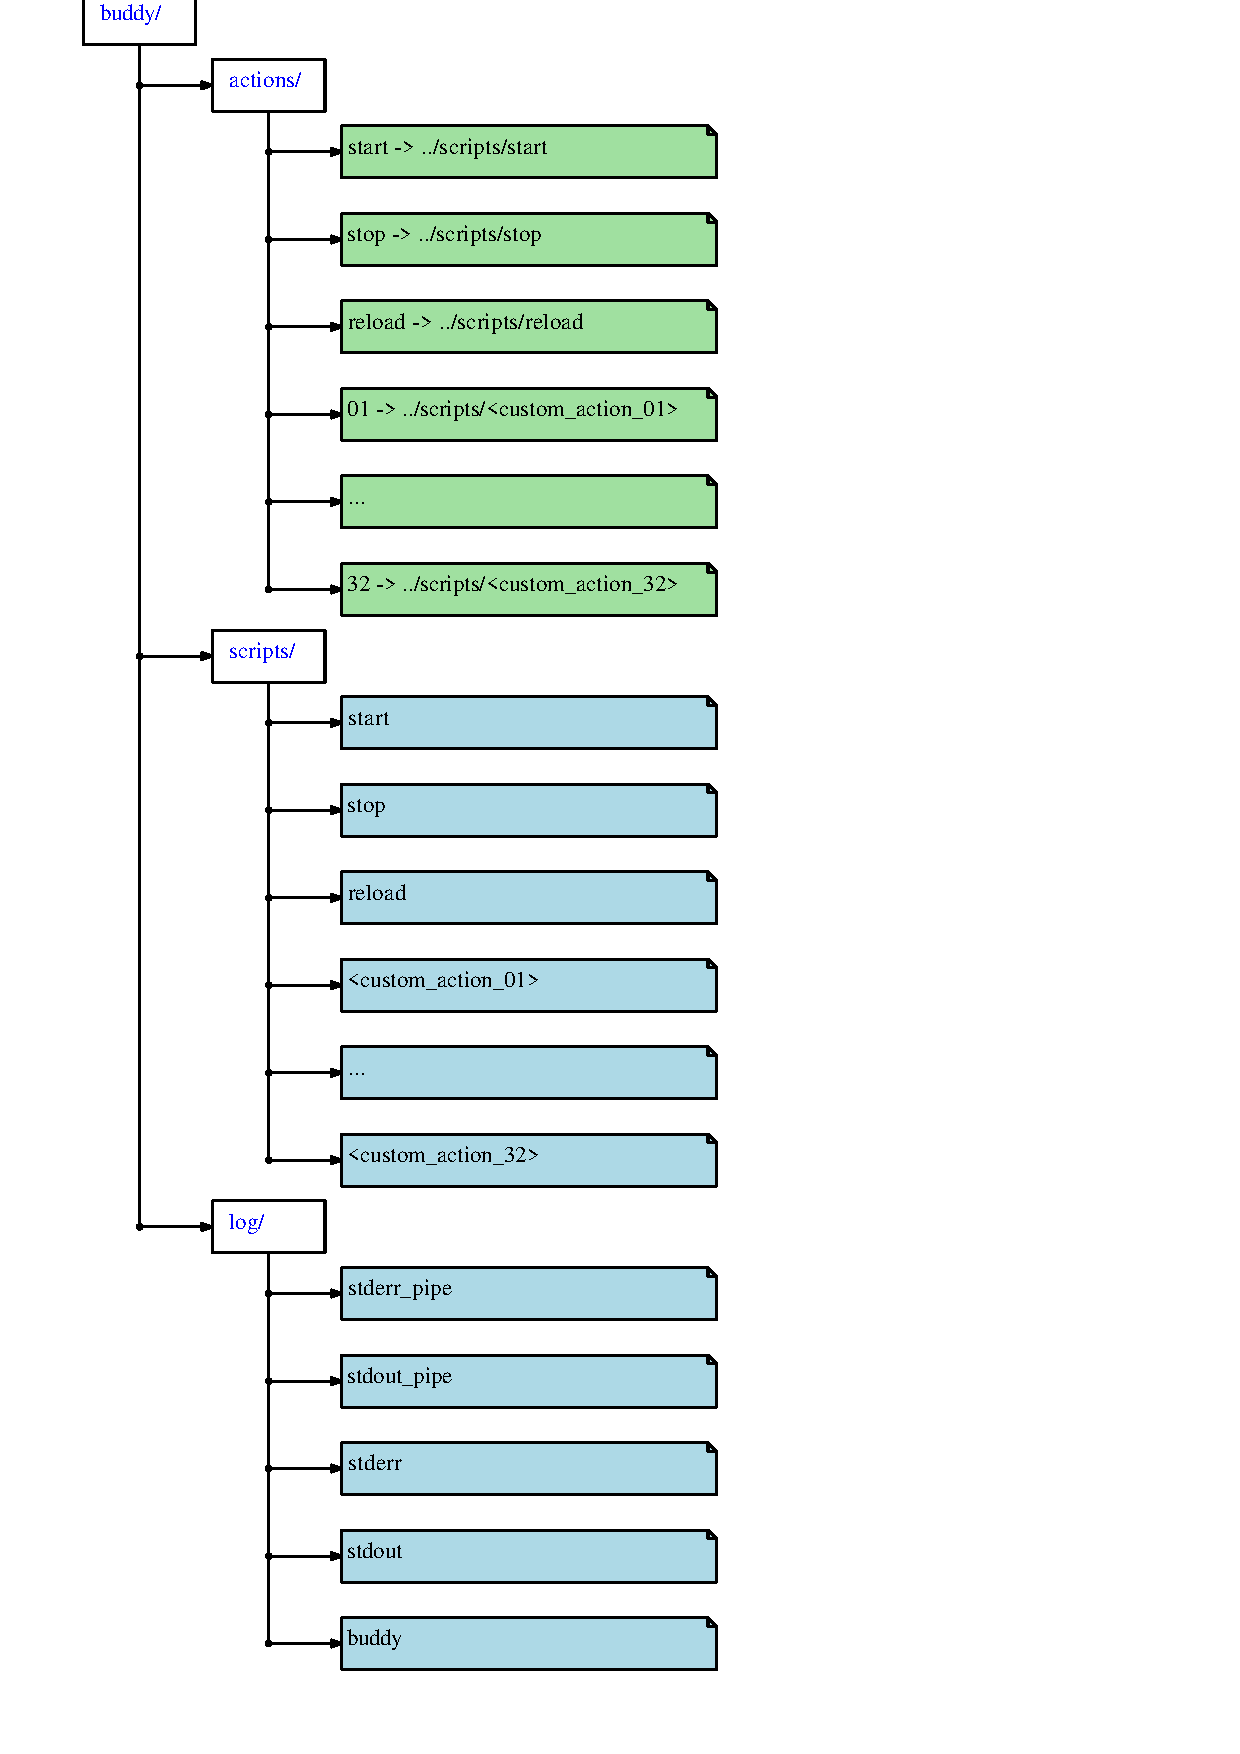
\includegraphics[width=\textwidth]{dot_inline_dotgraph_2}}
\end{DoxyImageNoCaption}
\end{center}


Clients consist of things like \char`\"{}uptop\char`\"{}, which is a status reporting tool that is similar to the common \char`\"{}top\char`\"{} utility. Clients communicate with controller via the API provided in libupkeeper. Hence, you can easily create any client you require, including metrics reporting and/or monitoring and alerting systems.

To explain this, the following sequence chart demonstrates how the components interact:

Start a managed process:

\begin{center}

\begin{DoxyImageNoCaption}  \mbox{\includegraphics{inline_mscgraph_1}}
\end{DoxyImageNoCaption}
\end{center}


Whereas a read-\/only process, such as subscribing to, and receiving events over time would look like this:

\begin{center}

\begin{DoxyImageNoCaption}  \mbox{\includegraphics{inline_mscgraph_2}}
\end{DoxyImageNoCaption}
\end{center}
\section{Sample Configuration.}\label{index_sampleconfig}
\begin{DoxyVerb}
{
    // StateDir
    // Path to variable state-dir for controller and buddies
    "StateDir": "/usr/var/upkeeper",

    // SvcConfigPath
    // Path to location of service configuration files
    "SvcConfigPath": "/usr/etc/upkeeper.d",

    // SvcRunPath
    // Path to location to setup and run buddies
    "SvcRunPath": "/usr/var/upkeeper/buddies",

    // Path to the buddy executable
    "UpkBuddyPath": "/usr/libexec/upk_buddy",

    // How frequently buddy sockets should be polled for events
    // in seconds and fractions of a second
    "BuddyPollingInterval": 0.5,

    // ServiceDefaults:
    "ServiceDefaults": {
        // An array of strings (['foo','bar']) describing what this service provides. These are then used in ordering service
        // startup via prerequisites. Service name, package, and UUID are implicitely added to the list of Provides.
        "Provides": [],

        // A valid UUID for the service, will be automatically generated if not provided.
        "UUID": Null,

        // A brief description of the service
        "ShortDescription": Null,

        // A longer and more complete description of the service
        "LongDescription": Null,

        // An array of strings (['foo','uuid#<...>']) of what must already be running (as named in 'Provides')
        // before this service should start. The syntax <package-name>:<service-name> may be used to specify a service from
        // a specific package. The syntax 'uuid#<uuid-string>' can be used to specify an explicit UUID.
        "Prerequisites": [],

        // Numeric start priority, used in lieu of, or in conjunction with Provides/Prerequisites to determine start order
        "StartPriority": 0,

        // Shutdown timeout before resorting to SIGKILL, Values < 0 will never SIGKILL
        "KillTimeout": 60,

        // Maximum number of times a process may fail in-a-row before its state is changed to down
        // a negative value indicates to restart forever (and is the default)
        "MaxConsecutiveFailures": -1,

        // user-defined max number of restarts within restart window
        "UserMaxRestarts": Null,

        // User-defined restart window, in seconds
        "UserRestartWindow": Null,

        // duration, in seconds, to wait between respawn attempts
        "UserRateLimit": Null,

        // a flag to enable/disable adding a randomized jitter to the user_ratelimit
        "RandomizeRateLimit": false,

        // if controller and/or buddy is run euid root; which uid to run the service as
        "SetUID": 0,

        // if controller and/or buddy is run euid root; which gid to run the service as
        "SetGID": 0,

        // size of the ringbuffer to maintain in the buddy
        "RingbufferSize": 64,

        // number of times to retry connections to the controler when emergent actions
        // occur in the buddy; (-1 for indefinate)
        "ReconnectRetries": 10,

        // command to exec for start, see 'StartScript'
        "ExecStart": Null,

        // script to start the monitored process; The default is 'exec %(EXEC_START)'
        "StartScript": "#!/bin/sh\nexec %(EXEC_START)\n",

        // command to exec for stop. Default: 'kill', see 'StopScript'
        "ExecStop": "kill",

        // Script to stop the monitored process. The default is 'exec %(EXEC_STOP) $1'; where $1 passed
        // to it will be the pid of monitored process (and also the pgrp, and sid, unless the monitored process changed them
        "StopScript": "#!/bin/sh\nexec %(EXEC_STOP) $1\n",

        // command to exec for reload. Default: 'kill -HUP', see 'ReloadScript'
        "ExecReload": "kill -HUP",

        // Script to reload the monitored process. The default is 'exec %(EXEC_RELOAD) $1'; where $1 passed
        // to it will be the pid of monitored process (and also the pgrp, and sid, unless the monitored process changed them
        "ReloadScript": "#!/bin/sh\nexec %(EXEC_RELOAD) $1\n",

        // A collection of key/value (JSON Object: {"foo":"bar"}) pairs where the key is the name of the action, and
        // the value is the contents of a script script to run for that action
        "CustomActions": {},

        // optional script to pipe stdout to. For example: 'exec logger -p local0.notice'
        "PipeStdoutScript": Null,

        // optional script to pipe stderr to. For example: 'exec logger -p local0.warn'
        "PipeStderrScript": Null,

        // optional place to direct stdout.
        // Note that if you pipe stdout elsewhere, this might never be written to, unless the thing you pipe to prints
        // to stdout itself
        "RedirectStdout": Null,

        // optional place to direct stderr.
        // Note that if you pipe stderr elsewhere, this might never be written to, unless the thing you pipe to prints
        // to stderr itself
        "RedirectStderr": Null,

        // state the service should be set to initially. this is used only when a service is first configured.
        "InitialState": "stopped",

        // May be used by a package to instruct the controler to remove a configured service
        // if the file defining that service ever disappears. Possibly useful in packaging
        // to cleanup the controller on package removal. The default behavior is to ignore
        // file removal, and require explicit manual removal of configured services
        "UnconfigureOnFileRemoval": false,

        // If the controller starts/restarts, and buddy has a service state set to 'stopped',
        // but controller's data-store believes the service should be running, prefer
        // buddy's world view, and update the data-store to reflect the stopped state.
        // The default is to trust the data-store; which would cause the service to be started
        "PreferBuddyStateForStopped": false,

        // if the controller starts/restarts, and buddy has a service state set to 'running',
        // but controller's data-store believes the service should be stopped, prefer
        // buddy's world view, and update the data-store to reflect the running state.
        // The default is to trust the buddy, which would leave the service running
        "PreferBuddyStateForRunning": true,
    },
}
\end{DoxyVerb}
 